\chapter{绪论}

\section{研究动机}
如今 Web 上的内容每天都在以指数级的速度增长\cite{limaye2010annotating},这也使得 Web 近年来成为世界上最大的数据集散地之一。
据估计 Web 上有超过141亿张表格,其中1.54亿张表格包含关系型数据并且仅 Wikipedia 就是大约160万关系型表格的来源。
可见Web 表格,换句话说是 Web 上的 HTML 表格,是关系型数据的一个重要来源和信息抽取 (Information Extraction) 系统的一个重要输入。
与普通文本不同,单张关系型表格就包含一系列高质量的关系实体并且在表格的表头中包含与实体相关的元数据。
Web 上包含关系型数据的表格中蕴含的巨大财富和价值使得表格的语义解释 (Semantic Interpretation),也就是将 Web 表格转换成机器能够理解的知识这一任务成为热门的研究领域。\par

另一方面,诸如维基百科等知识共享社区的蓬勃发展和信息抽取技术的进步已经促成了大规模机器可读知识库的自动化建设。
目前世界上已经出现了上百个领域不同、规模不一的知识库 (Knowledge Base) 并且它们的规模每天都在飞速增长。知识库中包含着整个世界的实体,实体的语义类别及其相互关系的丰富信息。
这样典型的例子包括 YAGO\cite{suchanek2007yago},DBpedia\cite{auer2007dbpedia} 和 Freebase\cite{bollacker2008freebase}。
在中文知识库中较有影响力的就是由上海交通大学和东南大学共同建立的 Zhishi.me\cite{niu2011zhishi}。\par

Web 上虽然蕴含着许多有价值的数据,但更多的却是各种原始并且充斥着噪声的数据,其中有些甚至是错误的。
这些数据大都是以自然语言的形式存在,然而由于自然语言表达的多样性与歧义性,使得它们很难被计算机直接处理或者理解。
面对如此规模庞大而嘈杂的数据,信息过载的现象每天都在发生。
信息过载意味着在找到想要的有用的信息之前,需要处理大量的无用数据,计算机获取有效信息的效率常常受到限制。
为了减轻信息过载带来的负面影响以及处理自然语言的多样性问题和歧义性问题,语义网 (Semantic Web) 的概念应运而生,旨在对现有万维网上的文档进行元数据 (Meta Data) 标注,使计算机能够理解词语和概念以及它们之间的逻辑关系。
将 Web 数据与知识库链接起来是非常有利于标注 Web 上的大规模数据的,并且有助于实现语义网的愿景\cite{berners2001semantic}。
许多为了解释说明 Web 表格内含的语义的研究工作\cite{limaye2010annotating}\cite{hignette2009fuzzy}\cite{mulwad2013semantic}\cite{munoz2014using}\cite{syed2010exploiting}\cite{venetis2011recovering}是将其内容标注成 RDF 三元组。
这种语义标注 (Semantic Annotation) 的关键一步就是实体链接 (Entity Linking),将出现在 Web 表格单元格中的字符串指称 (Mention) 链接到其在给定知识库中对应的参考实体 (Entity)。\par

实体链接技术的发展可以带动许多不同的应用的发展,比如知识库补全,自然语言问答系统和语义搜索系统。
随着社会的发展,新的知识被创造出来并以数据的形式表现在 Web 上。
因此,利用这些新知识扩充现有的知识库显得越发重要。
然而,为了将这些新知识插入到现有知识库中,会不可避免地需要一个系统,来将字符串指称,也就是与已抽取出的知识相关联的指称,链接到知识库中的相应实体。
例如,自然语言问答系统依靠它们支持的知识库来回答用户的问题。
为了回答``苹果公司创始人史蒂夫·乔布斯的诞生日期是哪天''这个问题,该系统应首先利用实体链接技术将查询语句中的``史蒂夫·乔布斯''映射到美国企业家,而不是美国传记电影,
然后从知识库中直接取回名为``史蒂夫·乔布斯''的出生日期。
除此之外,实体链接对数据集成很有帮助,可以将不同页面、文档和站点上的实体信息进行集成。
可见,Web 表格上的实体链接技术很有价值并且拥有广阔的应用前景。\par


\section{研究现状}

在本节中,我会回顾一些在 Web 表格上进行语义标注的相关研究工作,它们通常会处理三个任务:实体链接 (Entity Linking),列类型推理 (Column Type Inference) 以及关系抽取 (Relation Extraction)。 
在 Cafarella 等人\cite{cafarella2008webtables}报告说,有超过1.5亿个 Web 表格内嵌有高质量的关系型数据,许多研究人员意识到 Web 表格是许多应用的重要数据来源,比如信息抽取和结构化数据搜索。 
因此,与 Web 表格的语义标注相关的各种研究工作如雨后春笋般涌现出来。\par

Hignette 等人\cite{hignette2009fuzzy}提出了一种聚合的方法,使用给定本体中的词汇来标注 Web 表格中的内容。
它首先标注单元格,然后标注列的类型,最后标注列之间的关系。
与之相似的,Syed 等人\cite{syed2010exploiting}提出了一种管道方法,其首先进行列类型推理,然后将单元格的值链接到给定的知识库中的实体,最后选择列之间合适的关系。
Zhang \cite{zhang2014towards}设计了一个名为 TableMiner 的工具来标注 Web 表格。
TableMiner 只专注于列类型推理和实体链接,并不能从 Web 表格中抽取关系。
之后,Zhang \cite{zhang2014learning}又提出了一些策略来改进 TableMiner。 
Limaye 等人\cite{limaye2010annotating}和 Mulwad 等人\cite{mulwad2013semantic}提出了两种方法,可以分别对 Web 表格上的实体链接,列类型推理和关系抽取任务联合建模。
我的方法和这些研究工作之间的主要区别在于它不依赖任何特定的信息来完成实体链接的任务,例如 Web 表格的表头和标题,知识库中的实体类型和网页中的语义标记等等。\par

还有一些在特定场景下对 Web 表格进行语义标注的研究工作是没有实体链接的步骤的。
在 Venetis 等人\cite{venetis2011recovering}的研究工作中,他们的方法是弱化实体链接的影响,直接进行列类型推理,并且通过大规模的关系数据库 (Relation Databases) 中不同模式的出现频率来确定 Web 表格中的关系,这些关系数据库都是由网页构建的,但通常不对大部分研究人员开放。
此外,Munoz 等人\cite{munoz2014using}提出了一种从维基百科表格中挖掘 RDF 三元组的方法。
在这项研究中,他们能够通过内部链接和文章标题直接识别出维基百科中的实体。\par

跟我的方法最相近的研究工作是 Bhagavatula等人\cite{bhagavatula2015tabel} 和 Shen 等人\cite{shen2012liege}的研究工作。
Shen 等人\cite{shen2012liege}尝试将形如列表 (List-like) 的 Web 表格 (表格有多行但只有一列) 中的字符串指称链接到给定知识库中的实体。
Bhagavatula 等人\cite{bhagavatula2015tabel}提出了 TabEL,一个表格实体链接系统,它使用集体分类技术来对 Web 表格中的所有指称进行联合消岐 (Entity Disambiguation)。
这两个研究工作都不使用任何特定信息来进行实体链接,并且可以应用于任何知识库。
在本文中,为了提高 Web 表格中的实体链接的质量,我专注于在多个相互有链接关系的知识库下的实体链接而不是单个知识库下的实体链接。\par


\section{本文贡献}\label{contribution}

之前的 Web 表格实体链接研究中主要存在两个问题。
1) 许多研究工作\cite{limaye2010annotating}\cite{hignette2009fuzzy}\cite{mulwad2013semantic}\cite{syed2010exploiting}\cite{zhang2014towards}\cite{zhang2014learning}都非常依赖于基于特定信息的特征,
比如 Web 表格的表头 (e.g. ``电影'',``导演''等等。在图~\ref{el} 中表格的第一行中出现),目标知识库中的实体类型以及其他的一些特定信息。
假如我们要处理的 Web 表格中没有这样的表头信息抑或是给定的知识库中没有实体类型的信息,那么很显然前面提及的那些方法的效果会很有限。
2) 现在大部分实体链接的方法\cite{limaye2010annotating}\cite{hignette2009fuzzy}\cite{syed2010exploiting}\cite{zhang2014towards}\cite{zhang2014learning}\cite{shen2012liege}\cite{bhagavatula2015tabel}都只考虑将 Web 表格单元格中的字符串指称链接到单一知识库,但是每个知识库中的实体数量都是有限的,单一知识库无法保证在做 Web 表格上的实体链接的时候对实体有一个很好的覆盖度。
单知识库上的实体链接常常会出现实体缺失的状况。这个问题在这篇论文\cite{pereira2014entity}中的自然语言文本上实体链接的过程中也有体现。\par

为了克服上述问题,在我的毕业设计``基于多知识库的表格实体链接研究''中,我提出了两个新的通用的方法来做基于多知识库的 Web 表格实体链接。
1) 方法一中包含两个步骤。第一步是将一个不依赖于任何特定信息的基于图模型 (Probabilistic Graph Model) 的算法用来做 Web 表格与每个单知识库的实体链接。
然后在第二步中,我提出了三个启发式规则,利用来自不同知识库的实体之间的已存在的和新学习的 ``sameAs'' 关系,以提高第一步的实体链接结果的质量。
第二步不仅可以减少单知识库实体链接产生的错误,还可以提高实体链接结果的覆盖范围。
2) 方法二基于一种融合的思想,尝试用一个统一的图模型来表示 Web 表格中的字符串指称和来自多知识库的实体信息,然后在这个图模型上进行随机游走 (Random Walk),直接得到实体链接的结果。
简单的说,方法二融合了方法一中的两步,将多知识库间的 ``sameAs'' 关系加进了图模型,
同时也舍弃了方法一中的启发式规则,毕竟启发式规则是基于直觉和经验而定,在实际操作中有可能会因为多知识库间 ``sameAs'' 关系的缺失而舍弃一些非常有价值的实体链接结果,方法二规避了这些风险。
在实验中,我将一些 Web 表格样本中的字符串指称与 Zhishi.me\cite{niu2011zhishi} 中的实体进行链接,Zhishi.me 是最大的中文链接开放知识库,如图~\ref{zhishime_link} 所示,其由三个相互链接的中文在线百科知识库组成:中文维基百科\footnote{\url{https://zh.wikipedia.org}},百度百科\footnote{\url{http://baike.baidu.com}}和互动百科\footnote{\url{http://www.baike.com}}。

针对本文中的两个方法,设计了一些对比试验来将它们和目前最先进的实体链接系统 (即 TabEL\cite{bhagavatula2015tabel} 和 LIEGE\cite{shen2012liege}) 进行各方面的比较。
实验结果表明,本文中提出的方法在 MRR(即 Mean Reciprocal Rank\footnote{\url{https://en.wikipedia.org/wiki/Mean_reciprocal_rank}} 平均倒数排名),准确率,召回率和 F1 值等评价指标上都表现得很不错。
实验中用到的表格语料库和算法的实现代码\footnote{\url{https://github.com/yanshengjia/link}}都是公开的,人工标注实体的表格数据同样也对未来的表格实体链接研究者开放。\par

% Fig
\begin{figure}[htbp]
\centering
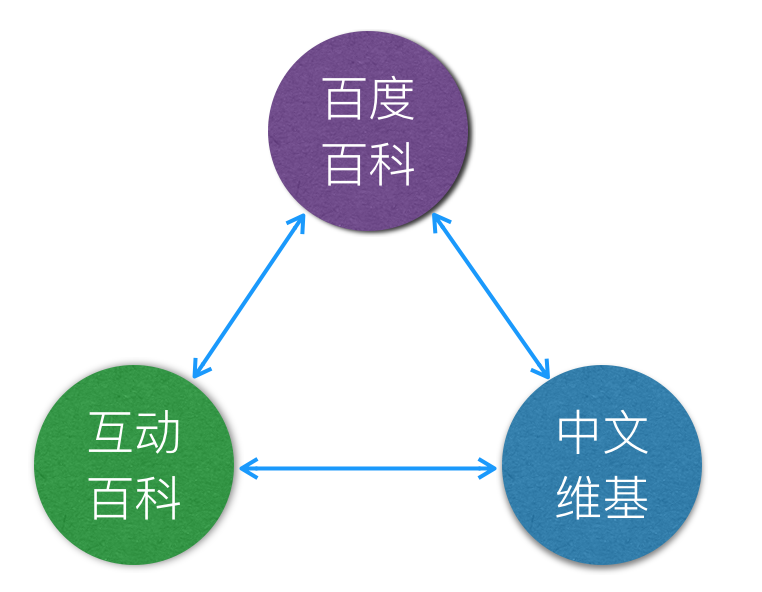
\includegraphics[width=0.4\textwidth]{img/zhishime_link}
\caption{Zhishi.me 由三个相互链接的知识库组成}
\label{zhishime_link}
\end{figure}

总而言之,本文的主要贡献在于:
\begin{enumerate}[1.]
  \item 提出了一个两阶段的基于多知识库的表格实体链接方法 (即方法一),并在实验中体现其比基于单一知识库的实体链接方法的优越性。该方法不依赖表格和知识库中的特定信息,而是建立了一个通用的图模型并使用随机游走算法来进行实体的迭代消岐。
  \item 提出了一个融合的支持多知识库的表格实体链接方法 (即方法二),其融合了方法一中的两步,规避了方法一中的启发式规则带来的风险,整个方法都是在一个统一的图模型上运行,一步到位得得出链接结果。
  \item 设计了一些对比试验,将本文提出的两个方法,TabEL\cite{bhagavatula2015tabel} 和 LIEGE\cite{shen2012liege} 在链接准确率、召回率、F1 值和 MRR 值上进行比较,从而验证本文提出的两个方法的效果。
  \item 在实体消岐时相较于以前的方法使用了很多十分具有价值的特征,比如字符串相似度特征、上下文相似度特征、同义词特征、三元组关系特征、知识库实体的消岐义特征等等。
  \item 添加了一些很有意义的功能,比如``sameAs'' 关系的学习。多知识库间的 ``sameAs'' 关系往往是不完备的,利用实体链接的结果可以与``sameAs''关系进行迭代学习,另外也可以通过监督学习分类器 SVM\cite{tong2001support} 进行``sameAs''关系的学习。
\end{enumerate}

本文的各章节内容是这样分配的:第一章是绪论的,介绍了我的毕设项目的研究动机、相关研究工作以及本文的主要贡献;
第二章从背景知识的角度出发阐述了基于多知识库的实体链接技术的方方面面,包括任务目标、关键挑战以及一般链接流程;
第三章详细介绍了我的毕设研究中提出的两个方法的思想以及相关模型;
第四章从算法具体实现的角度切入,以一个工程师的身份讲述实现细节;
第五章是实验与评估,详述了整个实验流程,将本文中的两个方法与 TabEL\cite{bhagavatula2015tabel} 和 LIEGE\cite{shen2012liege} 在不同评价指标上进行对比并分析;
第六章也就是最后一章总结了全文,并展望了未来工作。












